\documentclass[12pt, a4paper]{article}

\usepackage{amsmath}
\usepackage{array}
\usepackage[portuguese]{babel}
\usepackage{caption}
\usepackage{chngpage}
\usepackage{cite}
\usepackage{float}
\usepackage[a4paper, margin=2cm]{geometry}
\usepackage{graphicx}
\usepackage{hyperref}
\usepackage{longtable}
\usepackage{setspace}

\chardef\_=`_

\title{
    \vspace*{\fill}
    \textbf{
        Inteligência Artificial -- Trabalho Prático  \\
        \large Distribuição de alimentos durante uma catástrofe natural
    }
}

\author{
    \begin{tabular}{lc}
        Ana Carolina Penha Cerqueira       & A104188 \\
        Humberto Gil Azevedo Sampaio Gomes & A104348 \\
        João Pedro de Vasconcelos Torres   & A95748  \\
        José António Fernandes Alves Lopes & A104541 \\
        José Rodrigo Ferreira Matos        & A100612 \\
    \end{tabular}
}

\date{3 de janeiro de 2025 \vspace*{\fill}}

\captionsetup{font=onehalfspacing}

\begin{document}

\onehalfspacing
\setlength{\parskip}{\baselineskip}
\setlength{\parindent}{0pt}
\def\arraystretch{1.5}

\begin{titlepage}
    \maketitle
\end{titlepage}

\pagenumbering{gobble}
\pagebreak
\pagenumbering{arabic}

\section{Obtenção e representação do mapa}

O mapa da freguesia de São Vítor é obtido com uma \emph{query} à \emph{Overpass API}, do projeto
\emph{OpenStreetMap}, feita através da biblioteca Python \texttt{requests}. Foi desenvolvido um
sistema de \emph{caching} para não ser necessária a transferência do mapa no início todas as
execuções da aplicação desenvolvida. Do mapa, apenas são extraídas estradas (\texttt{way}s com a
\emph{tag} \texttt{highway}), e são ignorados todos os outros tipos de via.

O \emph{parsing} do XML obtido da \emph{query} à API é feito com as bibliotecas
\texttt{BeautifulSoup} e \texttt{lxml}. Nesta etapa, o mapa pode ser configurado como sendo um grafo
orientado (os sentidos das estradas devem ser respeitados) ou não (é possível dirigir em contramão).
No mapa da topologia apresentado, optou-se por esta segunda opção, uma vez que se considerou que o
código de estrada pode ser ignorado durante uma catástrofe natural onde são várias as estradas
cortadas.

Um grafo é armazenado como uma matriz de adjacência esparsa. Um dicionário associa nós (origens de
arestas) a outro dicionário, que associa nós (destinos de arestas) a custos. Por exemplo, a
expressão \texttt{edges[o][d] = c} quer dizer que existe uma aresta entre \texttt{o} e \texttt{d}
de custo \texttt{c}. Num mapa, \texttt{o} e \texttt{d} são inteiros, identificadores de nós na
base de dados do \emph{OpenStreetMap}, e \texttt{c} é um valor de vírgula flutuante. Um mapa
armazena também outro dicionário, que associa identificadores de nós às suas coordenadas. Estas,
durante a importação do mapa, são calculadas, de acordo com a projeção de Mercator, com base na
latitude e longitude de cada nó.

Por último, as condições meteorológicas num mapa são representadas por outro dicionário, que associa
arestas (pares origem-destino) a valores de vírgula flutuante entre 0.0 e 1.0, os extremos do bom e
do mau tempo, respetivamente. Para uma geração de condições meteorológicas em gradiente (sem grandes
picos ou vales nos valores), ruído Perlin (através da biblioteca Python \texttt{perlin-noise}) foi
utilizado.

\section{Algoritmos de procura}

Foram implementados diversos algoritmos de procura, para poderem ser comparados em aspetos de
qualidade da solução gerada e de desempenho computacional. Nesta secção, procura-se enumerar os
algoritmos implementados e descrever algumas das otimizações desenvolvidas.

\subsection{Procura em profundidade}

Este algoritmo foi implementado com algumas diferenças em relação à sua implementação
\emph{standard}. Em primeiro lugar, é armazenado um conjunto de nós visitados, que é utilizado para
garantir que o algoritmo termina, mesmo em grafos com ciclos. De seguida, o algoritmo também foi
implementado iterativamente, e não recursivamente. Devido ao grande tamanho de uma \emph{frame} da
\emph{stack} em Python, o limite de chamadas recursivas é bastante baixo, pelo que a implementação
iterativa se provou necessária para caminhos longos. Por último, o algoritmo não expande nós que
ultrapassem o limite de combustível do veículo a realizar a procura, diminuindo o número de nós
visitados quando não existe um caminho que o veículo seja capaz de realizar.

\subsection{Procura iterativa}

Este algoritmo, através de chamadas sucessivas ao algoritmo de procura em profundidade (com uma
profundidade máxima definida), encontra o caminho entre dois nós com o menor número de saltos. No
entanto, o algoritmo de procura em profundidade descrito anteriormente não pode ser utilizado para
uma procura iterativa. O uso de um conjunto para registar os nós visitados e evitar ciclos faz com
que, após \emph{back tracking}, alguns caminhos possíveis não sejam considerados, uma vez que
envolvem nós já visitados. Logo, a verificação de ciclos na procura em profundidade limitada é feita
através da consulta do caminho até ao nó atual (e se a sua expansão não causará um ciclo)
\cite{aima}. Esta verificação mais lenta e o maior número de nós visitados (é possível que o mesmo
nó seja visitado várias vezes) fazem com que este algoritmo exija um tempo de processamento muito
superior aos restantes, pelo que não será considerado para os testes realizados.

\subsection{Procura em largura}

Este algoritmo encontra o caminho entre dois nós com o menor número de saltos. Para um melhor
desempenho, foi usada uma lista duplamente ligada para a implementação da fila de espera deste
algoritmo. Deste modo, tanto as operações de \emph{push} como \emph{pop} podem ser executadas em
tempo constante. Tal como na procura em profundidade, o algoritmo não expande nós que ultrapassem o
limite de combustível do veículo a realizar a procura.

\subsection{Procura de custo uniforme / Algoritmo de Dijkstra}

Este algoritmo encontra o caminho com menor custo entre dois nós. Para a implementação da fila de
prioridades necessária para este algoritmo, foi utilizado um \emph{heap} binário, que apresenta
melhor desempenho do que listas. Tal como os outros algoritmos, não são expandidos nós fora do
alcance do combustível do veículo a realizar a procura, diminuindo o número de nós visitados quando
não existe um caminho que o veículo seja capaz de realizar.

\subsection{Procura gulosa}

Este algoritmo é muito semelhante à procura em profundidade, com a diferença de que a ordem de
expansão dos vizinhos de um nó é determinada por uma heurística. Tal como na implementação da
procura em profundidade, o algoritmo foi implementado iterativamente, e também não expande nós
fora do alcance do combustível do veículo a realizar a procura. Uma outra otimização, exclusiva à
procura gulosa, relaciona-se com a heurística de distância cartesiana. Como os valores da
heurística apenas são utilizados para comparação entre si, visto que a raiz quadrada é uma função
monótona crescente, o seu cálculo não é necessário, melhorando o desempenho do algoritmo:

$$
    dx_1^2 + dy_1^2 < dx_2^2 + dy_2^2
    \Rightarrow
    \sqrt{dx_1^2 + dy_1^2} < \sqrt{dx_2^2 + dy_2^2}
$$

\subsection{A*}

A única diferença entre este algoritmo e o algoritmo de Dijkstra é a ordem dos nós na fila de
espera, que passam a estar ordenados pela soma da sua distância à origem da procura com a sua
heurística. Quando a heurística é cartesiana, já não é possível evitar o cálculo das raízes
quadradas como na procura gulosa, visto que é necessário que a heurística não sobreestime o custo
entre dois nós caso se deseje que o algoritmo devolva a solução ótima de um problema de procura
\cite{aima}.

\subsection{Comparação dos algoritmos de procura}

Para comparar o desempenho e a qualidade das soluções dos vários algoritmos, estes foram executado,
no grafo apresentado, entre o centro de distribuição e os vários pontos de recolha de bens. Os
testes foram realizados com as condições meteorológicas desativadas, considerando um veículo de
alcance ilimitado. Ademais, foram testados todos os algoritmos com exceção da procura iterativa
(devido ao seu longo tempo de execução), e os algoritmos de procura informada foram testados com
duas heurísticas, uma baseada na distância cartesiana e a outra na distância de Manhattan. Foram
várias as métricas recolhidas, e os dados completos podem ser observados no anexo
\ref{comparison-data}. Aqui, apresentam-se as somas das métricas para todos os destinos,
procurando-se apresentar uma visão mais geral dos resultados obtidos:

\begin{table}[H]
    \small

    \begin{adjustwidth}{-1.5cm}{-1.5cm}
        \begin{center}
            \begin{tabular}{|l|r|r|r|r|}
                \hline
                                               &
                    $\Sigma_\text{Tempo}$ (ms) &
                    $\Sigma_\text{Custo}$      &
                    $\Sigma_{N\text{nós}}$     &
                    $\Sigma_{N\text{visitas}}$ \\

                \hline
                DFS & 72,78 & 196564,98 & 8408 & 31799 \\
                \hline
                BFS & 37,01 & 13118,15 & 356 & 29391 \\
                \hline
                Dijkstra & 97,58 & 12411,22 & 405 & 36109 \\
                \hline
                Greedy (Cart) & 73,47 & 40882,16 & 1805 & 12357 \\
                \hline
                Greedy (Man) & 52,14 & 20596,48 & 732 & 9468 \\
                \hline
                A* (Cart) & 25,58 & 12411,22 & 405 & 7570 \\
                \hline
                A* (Man) & 7,67 & 12596,46 & 428 & 2830 \\
                \hline
            \end{tabular}
        \end{center}
    \end{adjustwidth}

    \caption{Somas das diversas métricas recolhidas nos testes dos vários algoritmos de procura.}
\end{table}

Como esperado, tanto o algoritmo de Dijkstra como o A* (com heurística cartesiana) são capazes de
encontrar as soluções ótimas dos problemas de procura. No entanto, o A* não exige nem tanto tempo de
execução nem tanta memória, uma vez que o uso da heurística regula a ordem de visita dos nós e
permite que um menor número destes tenha de ser visitado.

Quando o A* é utilizado com a heurística baseada na distância de Manhattan, nem sempre resulta na
solução ótima. Isso é esperado, visto que apenas é garantido que o algoritmo A* seja ótimo quando
a heurística não sobreestima o custo entre nós \cite{aima}, o que não é verdade com a distância de
Manhattan. No entanto, esta heurística é de cálculo mais rápido e, no grafo utilizado, reduz o
número de nós visitados significativamente, diminuindo consideravelmente o tempo de execução e o uso
de memória do A* (quando comparado com a heurística cartesiana). Considerando isto e o facto de que
as soluções obtidas apresentam um custo muito próximo do ótimo, este algoritmo é o que melhor
equilibra entre tempo de execução e qualidade da solução.

Nos problemas de procura apresentados, caso não fosse possível implementar algoritmos de procura
informada, a procura em largura não seria uma má escolha de algoritmo. Ao contrário do algoritmo de
Dijkstra, a procura em largura não é ótima, visto que o grafo é pesado. No entanto, as soluções
encontradas são próximas da ótima, e tanto o tempo de processamento necessário como os requisitos de
memória (número de visitas) são menores do que os do algoritmo de Dijkstra, tornando este algoritmo
viável caso a solução ótima não seja necessária. Uma forma de obter a solução ótima com a procura em
largura seria uma pré-discretização do grafo, ou seja, inserir nós em arcos longos para garantir que
todos os arcos têm o mesmo custo / comprimento.

Por último, os algoritmos de procura em profundidade e de procura gulosa foram os que apresentaram
as piores soluções, visto que não têm em consideração o custo das soluções encontradas, e apenas se
"preocupam"{} com arranjar uma solução válida. A procura gulosa, devido ao uso de uma heurística,
gera, a partir da origem, caminhos na direção do destino, diminuindo o seu comprimento (e
consequentemente o custo da solução) e o número de nós visitados (requirindo menos memória). Por
outro lado, a procura em profundidade, como não utiliza uma heurística, várias vezes gera uma
solução que consiste em dar uma "volta"{} ao mapa antes de chegar ao destino.

\section{Algoritmo para empacotamento}

Para o envio de recursos para um local, é necessário distribuí-los por veículos, Surge um problema
de empacotamento, onde se procura distribuir vários produtos, cada um com um peso, por vários
veículos, cada um com um limite de peso e um custo de envio, procurando maximizar-se o peso enviado,
enquanto se minimiza o custo de envio dos veículos.

Na aplicação desenvolvida, este problema é resolvido com um algoritmo genético. Um indivíduo, que
correspondente a uma distribuição dos produtos pelos veículos, é constituído por tantos genes
quantos produtos. Cada gene é um número inteiro, e corresponde ao veículo em que o produto deve ser
colocado. Segue-se, abaixo, o exemplo de um indivíduo, onde todos os produtos são colocados no
veículo 0, com exceção do 3º produto, que é colocado no veículo 1.

\begin{table}[H]
    \begin{center}
        \begin{tabular}{|c|c|c|c|c|}
            \hline 0 & 0 & 1 & 0 & 0 \\ \hline
        \end{tabular}

        \caption{Exemplo um indivíduo no algoritmo genético utilizado para empacotamento.}
    \end{center}
\end{table}

A função de \emph{fitness} utilizada devolve 0 caso pelo menos um dos veículos ultrapasse o seu
limite de preço. Quando esta condição não é violada, procura-se, por esta ordem, maximizar o
peso enviado, minimizar o custo dos veículos enviados, e minimizar o número de veículos enviados.
Para ordenar estes valores, garantiu-se, através de multiplicações, que estes estavam em diferentes
ordens de grandeza:

$$
\mathcal{F}(X) =
\begin{cases}
    0
        ,& \text{se há veículos sobrecarregados} \\
    \text{Peso}(X) \times 10^6 - \text{Custo}(X) - \text{N}_\text{veículos}(X)
        ,& \text{caso contrário}
\end{cases}
$$

A operação de cruzamento é simples: é escolhido um índice onde os cromossomas dos pais são
divididos, e geram-se dois filhos, cada um com uma primeira parte do cromossoma de um dos pais e com
uma segunda parte do outro. A função de mutação, no entanto, já é mais complexa. Uma possível
mutação é a alteração do veículo no qual um produto é colocado. No entanto, para evitar que o
algoritmo convirja para colocar todos os produtos num veículo de maior custo quando um de menor
custo existe, uma possível mutação é a alteração de veículo de todos os produtos no mesmo veículo.

\section{Apresentação da solução do problema}

Quando a aplicação desenvolvida inicia, conforme os argumentos providenciados, pode ser gerada uma
solução de um problema de distribuição, ou pode ser carregada uma solução de um ficheiro. Em ambos
os casos, a solução será apresentada ao utilizador na interface que se procura descrever nesta
secção. Esta interface foi desenvolvida com recurso à biblioteca \texttt{pygame}.

Inicialmente, é apresentado o mapa com o centro de distribuição e os pontos de recolha. A tecla
\texttt{W} pode ser utilizada para alternar entre mostrar as condições meteorológicas ou não.
As setas do teclado podem utilizadas para mover o mapa na janela, e tanto o \emph{scroll} do rato
como as teclas \texttt{+} e \texttt{-} podem ser utilizadas para controlar o fator de ampliação.
Clicar num nó resulta na impressão de uma hiperligação para a saída textual do programa. Esta
hiperligação redireciona o utilizador para o \emph{Open Street Maps}, permitindo que este veja em
maior detalhe o mapa associado ao grafo apresentado.

\begin{figure}[H]
    \centering
    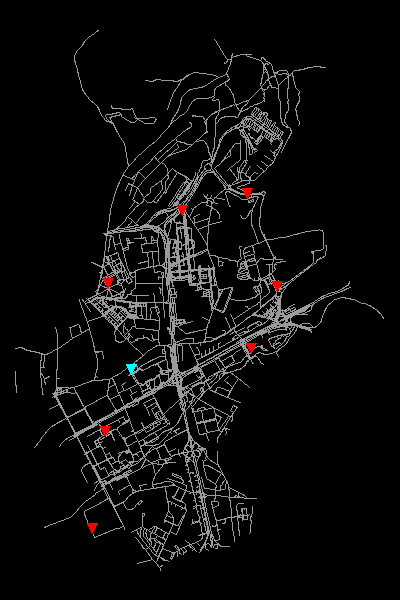
\includegraphics[width=0.45\textwidth]{res/PontosImportantes.png}
    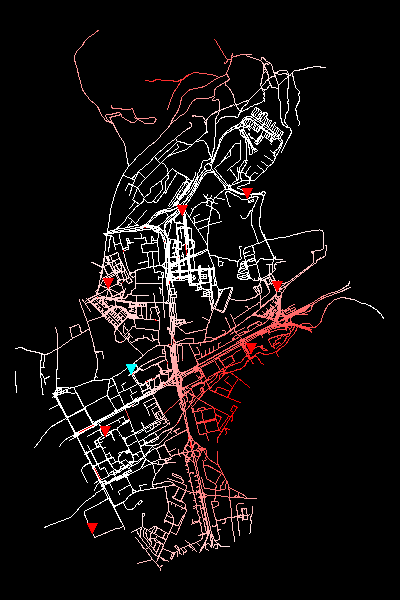
\includegraphics[width=0.45\textwidth]{res/Tempo.png}
    \caption{
        Apresentação do centro de distribuição e dos pontos de recolha na UI, sem e com condições
        meteorológicas visíveis.
    }
\end{figure}

As teclas \texttt{Enter} e \texttt{Backspace} são utilizadas para navegar entre os diapositivos da
apresentação da solução. Um diapositivo possível é a apresentação dos resultados de um algoritmo de
procura. O caminho, quando existente, é apresentado a azul, e os nós visitados são apresentados a
vermelho. Quando premida a tecla \texttt{A}, a interface anima o funcionamento do algoritmo,
mostrando os nós pela ordem que foram visitados.

\begin{figure}[H]
    \centering
    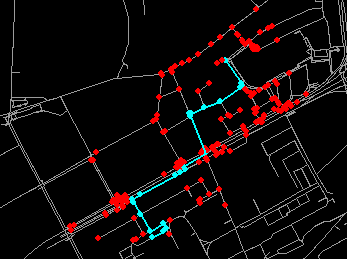
\includegraphics[width=0.45\textwidth]{res/Procura.png}
    \caption{Apresentação dos resultados de um algoritmo de procura na UI.}
\end{figure}

A interface também é capaz de apresentar o resultado do algoritmo de empacotamento, a satisfação de
entregas aos pontos de recolha, e a incapacidade de satisfazer um ponto de recolha a tempo.

\begin{figure}[H]
    \centering
    \begin{minipage}{0.32\textwidth}
        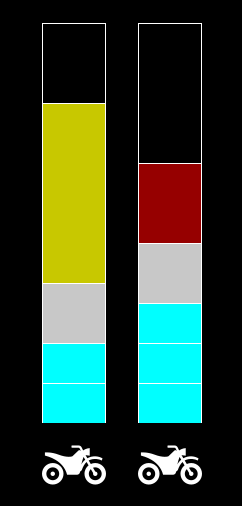
\includegraphics[width=\textwidth]{res/Empacotamento.png}
    \end{minipage}
    \begin{minipage}{0.45\textwidth}
        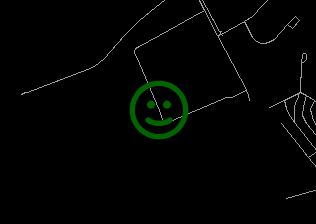
\includegraphics[width=\textwidth]{res/Sucesso.png}
        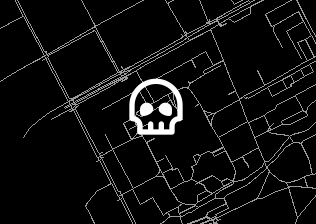
\includegraphics[width=\textwidth]{res/Morte.png}
    \end{minipage}
    \caption{
        Apresentação dos resultados do algoritmo de empacotamento, da satisfação de uma entrega a um
        ponto de recolha, e da incapacidade de satisfazer um ponto de recolha a tempo.
    }
\end{figure}
\section{Conclusão}

\section{Bibliografia}
\def\refname{}
\vspace{-1.5cm}
\begin{thebibliography}{9}
    \bibitem{aima} S. Russel and P. Norvig, \emph{Artificial Intelligence -- A Modern Approach},
        4th ed. USA: Pearson, 2021.
\end{thebibliography}

\section{Anexos}

\subsection{Resultados da comparação dos algoritmos de procura}
\label{comparison-data}

\begin{table}[H]
    \small

    \begin{adjustwidth}{-1.5cm}{-1.5cm}
        \begin{center}
            \begin{tabular}{|l|r|r|r|r|r|r|r|r|}
                \hline
                    Tempo (ms)  &
                    Tribunal    &
                    ESAS        &
                    INL         &
                    Cemitério   &
                    UMinho      &
                    Olimpo      &
                    Happy China &
                    $\Sigma$    \\

                \hline
                DFS & 0,54 & 21,73 & 6,32 & 15,55 & 6,99 & 10,06 & 11,59 & 72,78 \\
                \hline
                BFS & 1,09 & 4,85 & 2,35 & 3,11 & 7,24 & 9,87 & 8,5 & 37,01 \\
                \hline
                Dijkstra & 5,87 & 18,69 & 10,04 & 8,24 & 16,59 & 20,87 & 17,28 & 97,58 \\
                \hline
                Greedy (Cart) & 0,2 & 55,76 & 0,37 & 15,53 & 0,84 & 0,45 & 0,32 & 73,47 \\
                \hline
                Greedy (Man) & 0,14 & 0,52 & 0,33 & 49,75 & 0,78 & 0,37 & 0,25 & 52,14 \\
                \hline
                A* (Cart) & 0,65 & 2,55 & 1,61 & 3,25 & 1,62 & 12,85 & 3,05 & 25,58 \\
                \hline
                A* (Man) & 0,36 & 1,35 & 1,17 & 2,55 & 0,54 & 1,04 & 0,66 & 7,67 \\
                \hline
            \end{tabular}
        \end{center}
    \end{adjustwidth}

    \caption{
        Tempo de CPU para a execução de cada algoritmo de procura, entre o Bar Académico e os
        destinos apresentados.
    }
\end{table}

\begin{table}[H]
    \small

    \begin{adjustwidth}{-1.5cm}{-1.5cm}
        \begin{center}
            \begin{tabular}{|l|r|r|r|r|r|r|r|r|}
                \hline
                    Custo       &
                    Tribunal    &
                    ESAS        &
                    INL         &
                    Cemitério   &
                    UMinho      &
                    Olimpo      &
                    Happy China &
                    $\Sigma$    \\

                \hline
                DFS & 5315,16 & 4970,64 & 32428,01 & 40269,65 & 28219,21 & 42881,52 & 42480,79 & 196564,98 \\
                \hline
                BFS & 1010,32 & 2200,89 & 1683,98 & 1250,39 & 2242,19 & 2741,26 & 1989,12 & 13118,15 \\
                \hline
                Dijkstra & 1010,32 & 2158,87 & 1432,5 & 1250,39 & 1884,8 & 2717,2 & 1957,14 & 12411,22 \\
                \hline
                Greedy (Cart) & 1277,28 & 2305,31 & 2250,09 & 23491,25 & 4802,74 & 3797,38 & 2958,11 & 40882,16 \\
                \hline
                Greedy (Man) & 1291,62 & 2712,37 & 2671,13 & 2231,37 & 4934,5 & 3797,38 & 2958,11 & 20596,48 \\
                \hline
                A* (Cart) & 1010,32 & 2158,87 & 1432,5 & 1250,39 & 1884,8 & 2717,2 & 1957,14 & 12411,22 \\
                \hline
                A* (Man) & 1028,1 & 2179,62 & 1566,73 & 1250,39 & 1884,8 & 2717,2 & 1969,62 & 12596,46 \\
                \hline
            \end{tabular}
        \end{center}
    \end{adjustwidth}

    \caption{
        Custo das soluções dos vários algoritmos de procura, entre o Bar Académico e os destinos
        apresentados.
    }
\end{table}

\begin{table}[H]
    \small

    \begin{adjustwidth}{-1.5cm}{-1.5cm}
        \begin{center}
            \begin{tabular}{|l|r|r|r|r|r|r|r|r|}
                \hline
                    Nós na solução &
                    Tribunal       &
                    ESAS           &
                    INL            &
                    Cemitério      &
                    UMinho         &
                    Olimpo         &
                    Happy China    &
                    $\Sigma$       \\

                \hline
                DFS & 226 & 199 & 1384 & 1697 & 1157 & 1884 & 1861 & 8408 \\
                \hline
                BFS & 25 & 44 & 33 & 37 & 56 & 95 & 66 & 356 \\
                \hline
                Dijkstra & 25 & 68 & 35 & 37 & 74 & 96 & 70 & 405 \\
                \hline
                Greedy (Cart) & 45 & 49 & 91 & 1228 & 176 & 128 & 88 & 1805 \\
                \hline
                Greedy (Man) & 41 & 63 & 101 & 121 & 190 & 128 & 88 & 732 \\
                \hline
                A* (Cart) & 25 & 68 & 35 & 37 & 74 & 96 & 70 & 405 \\
                \hline
                A* (Man) & 26 & 58 & 68 & 37 & 74 & 96 & 69 & 428 \\
                \hline
            \end{tabular}
        \end{center}
    \end{adjustwidth}

    \caption{
        Número de nós nas soluções dos vários algoritmos de procura, entre o Bar Académico e os
        destinos apresentados.
    }
\end{table}

\begin{table}[H]
    \small

    \begin{adjustwidth}{-1.5cm}{-1.5cm}
        \begin{center}
            \begin{tabular}{|l|r|r|r|r|r|r|r|r|}
                \hline
                    Nós visitados &
                    Tribunal      &
                    ESAS          &
                    INL           &
                    Cemitério     &
                    UMinho        &
                    Olimpo        &
                    Happy China   &
                    $\Sigma$      \\

                \hline
                DFS & 255 & 8888 & 2881 & 6839 & 3136 & 4547 & 5253 & 31799 \\
                \hline
                BFS & 914 & 3857 & 2048 & 2593 & 5646 & 7738 & 6595 & 29391 \\
                \hline
                Dijkstra & 2379 & 6779 & 3909 & 3210 & 5929 & 7734 & 6169 & 36109 \\
                \hline
                Greedy (Cart) & 46 & 8885 & 99 & 2894 & 216 & 129 & 88 & 12357 \\
                \hline
                Greedy (Man) & 42 & 120 & 101 & 8766 & 221 & 130 & 88 & 9468 \\
                \hline
                A* (Cart) & 216 & 786 & 537 & 1061 & 519 & 3501 & 950 & 7570 \\
                \hline
                A* (Man) & 133 & 453 & 457 & 947 & 220 & 362 & 258 & 2830 \\
                \hline
            \end{tabular}
        \end{center}
    \end{adjustwidth}

    \caption{
        Número de nós visitados na execução dos vários algoritmos de procura, entre o Bar Académico
        e os destinos apresentados.
    }
\end{table}

\end{document}
